\section{One dimensional solution using freeform solution \label{SECTION_One dimensional solution using freeform solution}}
Optical cloaking of contact fingers has already been done in the following paper \cite{schumann2015cloaked}. With this technology, it is possible to cloak obstacles in one dimension, which are located between $x=0$ and $x=R_1$. In the paper \cite{schumann2015cloaked}, an analytical approximation in order to fulfil the optical properties is derived as well as an numerical solution. The analytical approximation is given in formula \ref{freeform_solution_oneD}. In this case, y(x) describes the boarder between the polymer (n=1.5) and air (n=1). 

\begin{align}
y(x)= \sqrt{y^2(0)+\frac{R_1}{1-\frac{1}{n}} \cdot \left(2x -\frac{x^2}{R_2} \right)} \label{freeform_solution_oneD}
\end{align}
\begin{figure}[h]
\centering
\includegraphics[width=\textwidth]{Martin_Schumann_paper.png}
\caption{source:\cite{schumann2015cloaked}[Fig. 2], One dimensional coordinate transformation x $\rightarrow$ x' of a point to a finite interval with width $2R_1$ leading to an angle distribution $\alpha (x)$. This distribution can be realized by a freeform surface y(x) of a dielectic with constant refractive index,n, on top of the solar cell. The local surface inclination angle is denoted by $\beta (x)$ \label{Martin_schumann_paper}}
\end{figure}

A picture of how the surface looks like can be found in figure \ref{Martin_schumann_paper}. In order to investigate in the advantages of the freeform solution, the optical cloak has been produced and tested. In one dimension they have shown that " transformed freeform polymer surfaces provide complete remedy of the shadowing problem. Potentially, these structures can be even mass manufactured." (\cite{schumann2015cloaked}[p. 853])

\section{Blending of the two one dimensional solutions}

Solar cells have on the sun-side two sorts of electrical contacts for collecting and transporting electrons. These are called busbars and contact fingers. The contact fingers and busbars are elongated perpendicular to each other. Usually, the busbars are larger than the contact fingers. 
From the section \ref{SECTION_One dimensional solution using freeform solution}, we know that cloaking in one direction turns out to work well. However, it is evident that a complete cloak of both, the contact fingers and the busbars, would lead to an optimal result. 
The first approach of the two dimensional problem is to investigate into an analytical solution. 
% KOMENTAR show that an analytical solution to the two dimensional problem cannot be achieved

Since it is shown that an analytical approach does not lead to a solution to the problem, we now want to blend the one dimensional solution in order to get a as good as possible solution. Different blendings are for instance:
\begin{align*}
z_1(x,y) &= a \cdot f(x) + b \cdot g(y) \\
z_2(x,y) &= f(x) \cdot g(y)
\end{align*}
We look at the performance for normal incidence and it turned out that the following solution fits best for normal incidence:
\begin{align}
z(x,y)= \sqrt{a \cdot  f(x)^2+b \cdot g(y)^2} \label{bledning_of_the_two_solutions}
\end{align}

\section{Simulation rectangular unit cell \label{SECTION_Simulation_rectangular_unit_cell}}
Most solar cells nowadays consist o rectangular unit cells. Therefore, we want first have a look at a rectangular unit cell. We chose the proportions of the cell with 1000 units in x direction and 100 units in y-direction. The x-scaling and y-scaling factors are set to be $sx=sy=0.9$. This means that $1-sx \cdot sy=19 $\% of the surface is covered with metal. The contact grid of the solar cell is indicated by the darker areas in figure \ref{contsurf_rectangular_normal_incident_planeofsolarcell}. The maximum possible annual improvement is $\xi_{max}= 23.46 $\%. 
\subsection{Optimised for normal incidence}

As you can see in formula \ref{bledning_of_the_two_solutions}, the parameters a and b can be chosen freely. In order to optimise the parameters, we first optimise the design for normal incidence. The fitness of a design describes how good a given design performs under chosen fitness- parameters. For fitness measurement for normal incidence, we take the number of rays and the average distance of the point the rays hitting the solar cell and their design point. With optimisation, we mean finding the parameter set for highest fitness of the design. 

\begin{table}[h]
\centering
\caption{Parameters for simulation for rectangular unit cell ( 500 x 50 units), optimisation means what constellation has been optimised (normalinc. means optimisation for normal incidence with number of rays on contact grid and average distance to deign point as fitness, annualimpr. means oprimisation for annual improvement using the annual improvement as fitness, only f(x)/g(y) is just the solution being perfect for x or y direction)}
\label{_table_rectangular_cell}
\begin{tabular}{c|c|c|c|c|c|c|c|c}
a & b & y0x & y0y & rx1 & ry1 & $\xi$+1 & optimisation & [nalphas,nbetas] \\
\hline\hline
2.07 & 5.00 & 49.77 & 55.54 & 51.00 & 9.46 & 1.1371 & annualImpr. & [10,10] \\
2.07 & 5.00 & 49.77 & 55.54 & 51.00 & 9.46 & 1.1101 & annualImpr. & [20,20] \\
1.9 & 2.0 & 75 & 70 & 50 & 5 & 1.1071 & normalinc. & [10,10] \\
1 & 0 & 50 & 0 & 50 & 0 & 1.1025 & only f(x) & [10,10] \\
0 & 1 & 0 & 5 & 0 & 5 & 1.0789 & only g(y) &[10,10]
\end{tabular}
\end{table}

\begin{figure}[h]
\centering
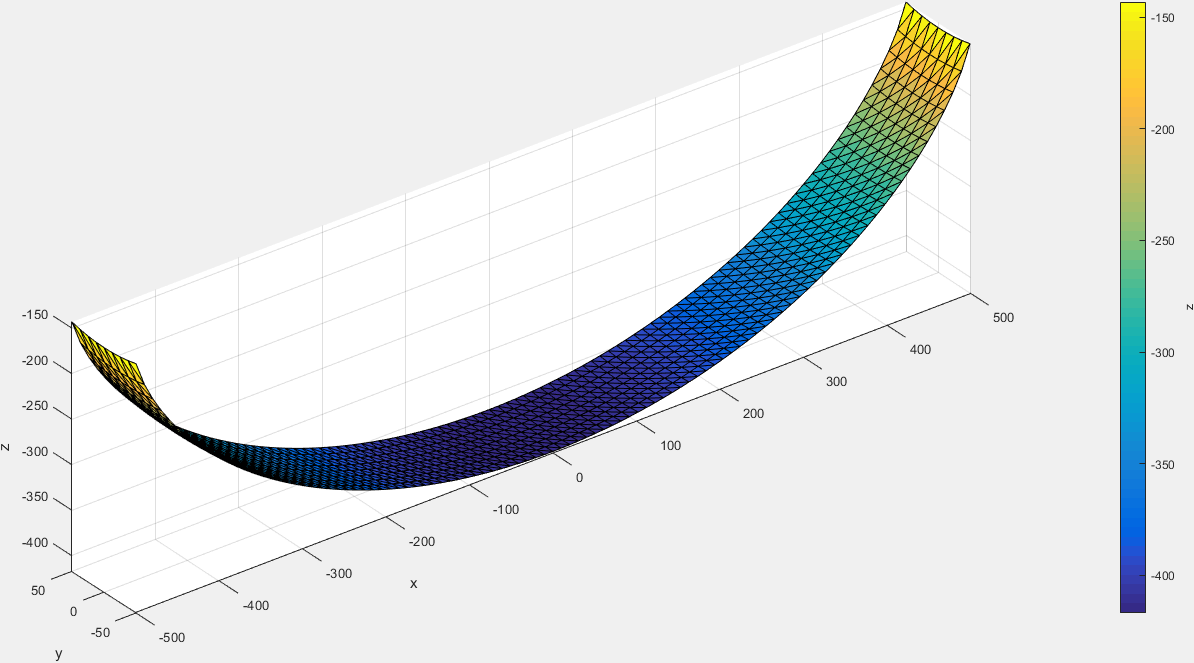
\includegraphics[width=\textwidth]{contsurf_rectangular_normal_incident_surface}
\caption{the solar cell is located at z=0 and the light is travelling in positive z direction, continuopus surface, rectangular solar cell, optimised for normal incidence \label{contsurf_rectangular_normal_incident_surface}}
\end{figure}

In order to get a feeling of how the freeform surface for a rectangular surface optimised for normal incident looks like, have a look at figure \ref{contsurf_rectangular_normal_incident_surface}. The solar cell sits at $z=0$ and the light is travelling into positive z-direction. You can see that the surface is bend a lot into the x-direction and hardly bend in the direction of y. It almost looks like the one dimensional solution in x-direction. 


\begin{figure}[h]
\centering
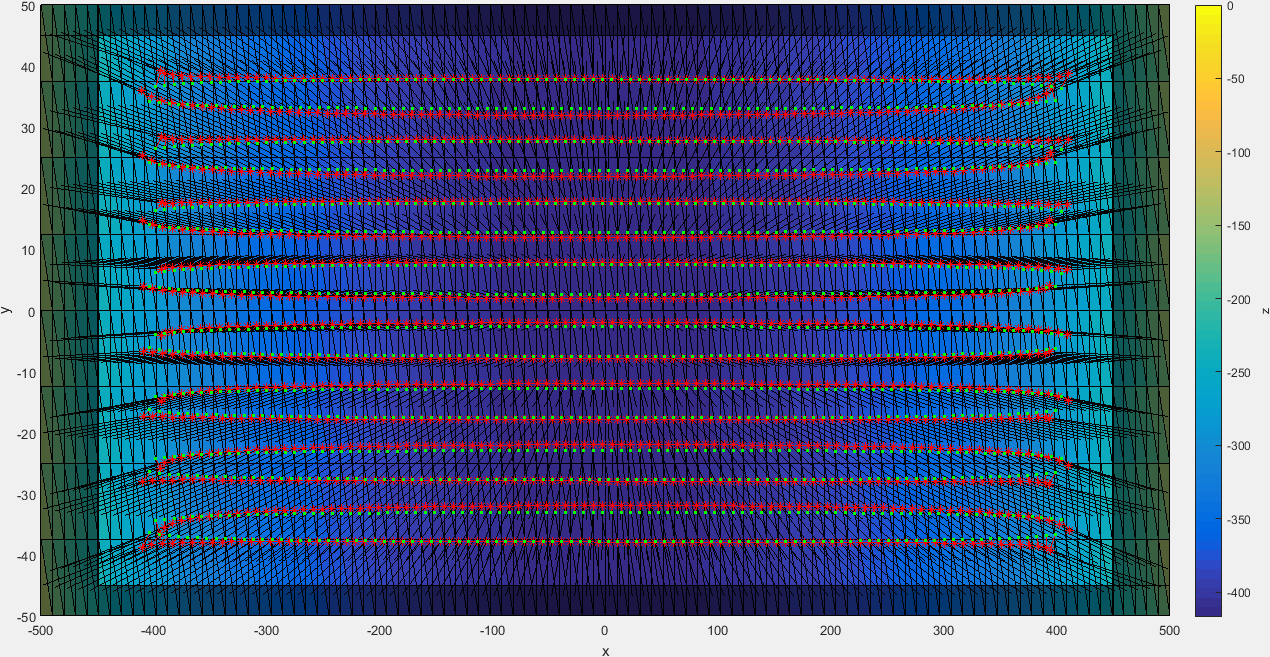
\includegraphics[width=\textwidth]{contsurf_rectangular_normal_incident_planeofsolarcell.png}
\caption{shows the average distance to the designpoint, continuopus surface, rectangular solar cell, optimised for normal incidence \label{contsurf_rectangular_normal_incident_planeofsolarcell}}
\end{figure}

In figure \ref{contsurf_rectangular_normal_incident_planeofsolarcell} you can see a projection to the plane of the solar cell. The dark areas in the figure show the contact grid of the solar cell. The figure shows one unit cell. Green dots are the design points and red points are the points the rays are hitting the solar cell. Each design point is connected with the corresponding point the rays hits the solar cell by a red line. You can see that qualitatively the design seems to work well for normal incidence since the design points and the points the rays hitting the solar cell are close to each other. However, for a more quantitative description, let us have a look at figure \ref{contsurf_rectangular_normal_incident_average_distance}. This figure shows the plane of the solar cell. For computational reasons, the surface has been triangulated. The colour of each triangle indicates the distance from the ray at this point to its design point. (see colour-bar on the right side of figure \ref{contsurf_rectangular_normal_incident_average_distance} for a more quantitative description ) The average distance from design point is 1.3 and the number of rays hitting the contact grid is 0. You can also notice that the design works quite well in the middle and quite bad on the edges. (bad performance for high and low x- values) 

\begin{figure}[h]
\centering
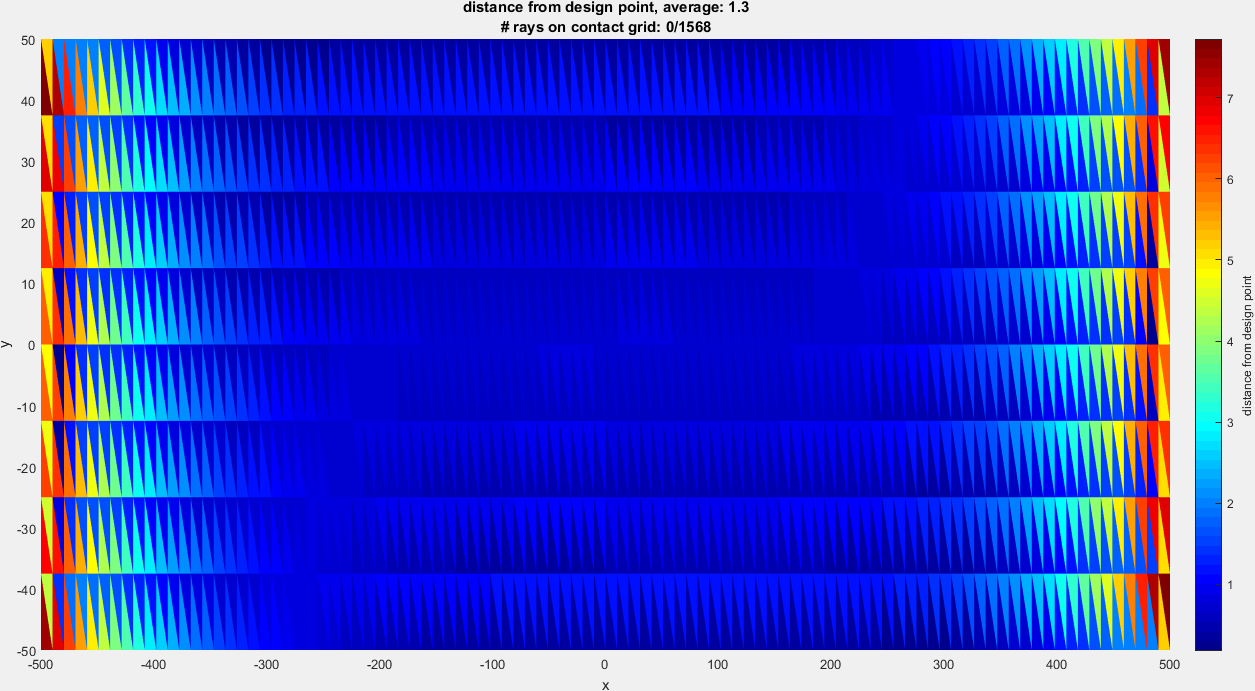
\includegraphics[width=\textwidth]{contsurf_rectangular_normal_incident_average_distance.png}
\caption{shows the average distance to the designpoint, continuopus surface, rectangular solar cell, optimised for normal incidence \label{contsurf_rectangular_normal_incident_average_distance}}
\end{figure}


Moreover, a better three dimensional understanding of the surface is needed. Therefore, let us have a look at figure \ref{contsurf_rectangular_normal_incident_view00}. This figure shows a x/z-projection of the polymer-structure with simulated rays. The light is travelling in positive z-direction. You can see that the rays around x=0 are hardly influenced by refraction and for high or small x-values, the surface of the polymer-structure is bend more and the rays are refracted under a higher angle. Qualitatively, the same happens for the üprojection into y/z-plane. (see figure \ref{contsurf_rectangular_normal_incident_view900}) Notice that the axis of figure \ref{contsurf_rectangular_normal_incident_view00} and \ref{contsurf_rectangular_normal_incident_view900} are not equal. You can see that the surface is bend a lot in x-direction and hardly bend in y-direction.  
Figure \ref{contsurf_rectangular_normal_incident_view3} shows a three dimensional image of the solar cell located at z=0 and the polymer structure. The light travels in positive z-direction. The contact grid is indicated by the gray rectangulars. 
The parameters used for this plots can be found in table \ref{_table_rectangular_cell}. For comparison we computed the annual improvement for all constellations. For optimisation for normal incidence this means a annual improvement of $10.71$ \%. This is 45,7 \% of the maximal annual improvement. In the next step, we search for a design with a as high as possible maximum improvement. 

\begin{figure}[h]
\centering
\begin{subfigure}{\textwidth}
\centering
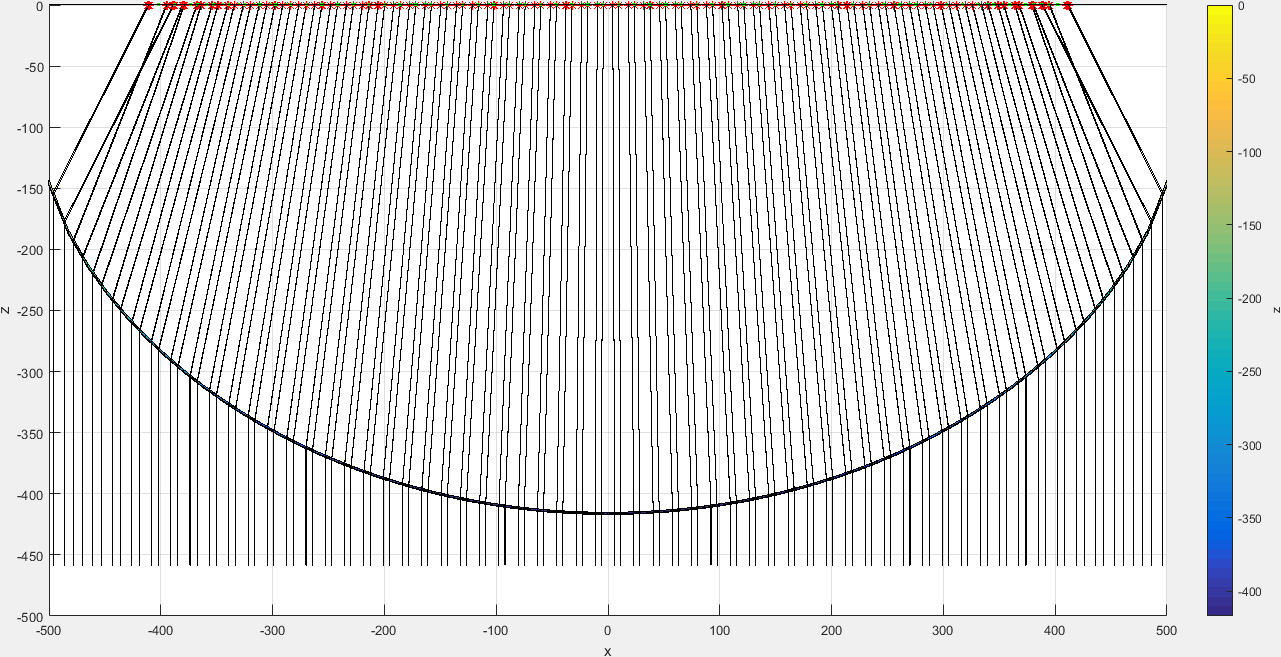
\includegraphics[width=0.48\textwidth]{contsurf_rectangular_normal_incident_view00}
\caption{\label{contsurf_rectangular_normal_incident_view00}}
\end{subfigure}
\begin{subfigure}{\textwidth}
\centering
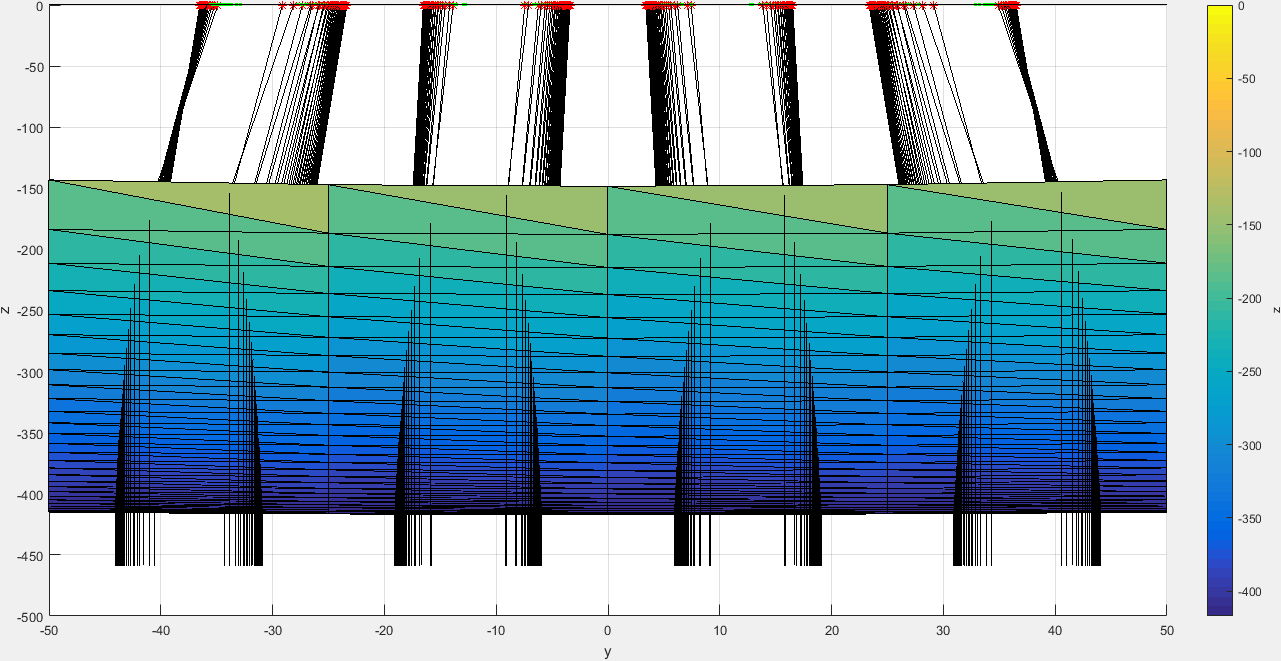
\includegraphics[width=0.48\textwidth]{contsurf_rectangular_normal_incident_view900.png}
\caption{ \label{contsurf_rectangular_normal_incident_view900}}
\end{subfigure}
\begin{subfigure}{\textwidth}
\centering
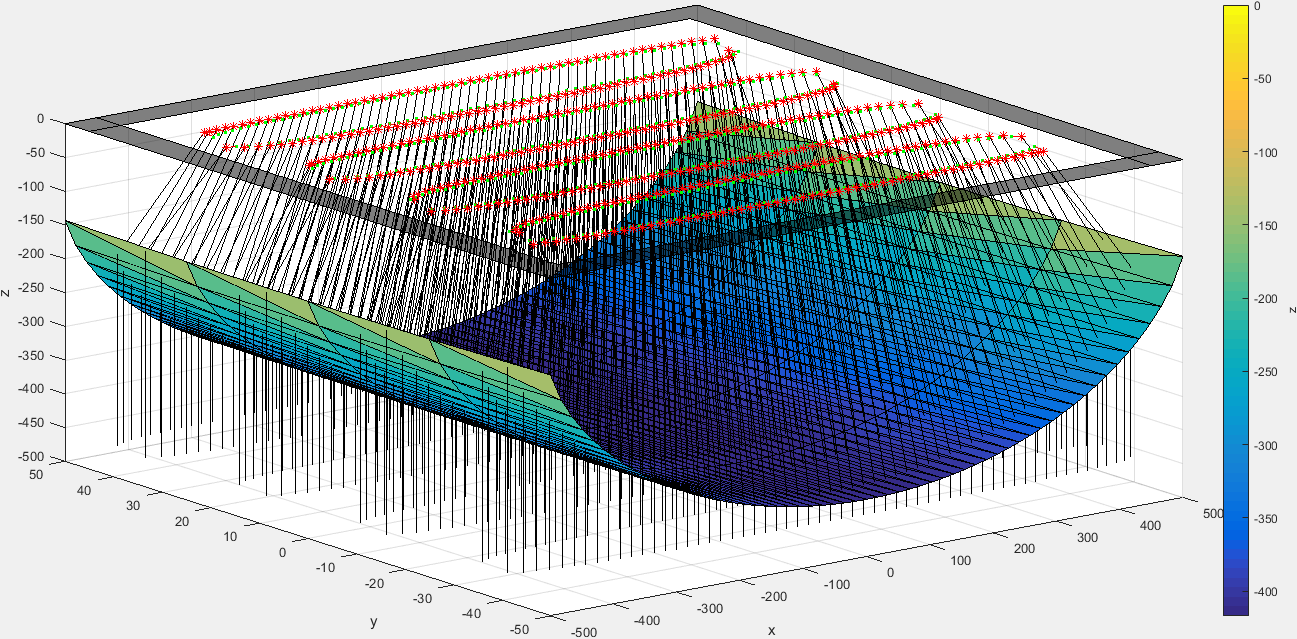
\includegraphics[width=\textwidth]{contsurf_rectangular_normal_incident_view3.png}
\caption{ \label{contsurf_rectangular_normal_incident_view3}}
\end{subfigure}
\caption{continuopus surface, rectangular solar cell, optimised for normal incidence, the solar cell is located at z=0 and the light is travelling in positive z direction}
\end{figure}

\clearpage

\subsection{Optimised for annual improvement}

The annual improvement of the surface optimised for normal incident reaches only 46 \% of the maximal annual improvement. We will try to enhance the annual improvement. It is possible that the design which works perfectly for normal incident does not give the best results for annual improvement. Therefore, we take the annual improvement itself as value for the fitness of the design. The annual improvement does not take the homogeneity of the light on the solar cell into account. The parameters for optimisation with the annual improvement as fitness can be found in table \ref{_table_rectangular_cell}. In figure \ref{contsurf_rectangular_annualopt_surface}, we can see the surface of one unit cell. Comparing figure \ref{contsurf_rectangular_annualopt_surface} (belonging to annual improvement) with figure \ref{contsurf_rectangular_normal_incident_surface} we notice that the figure belonging to annual improvement is bend a bit more in y-direction. 

\begin{figure}[h]
\centering
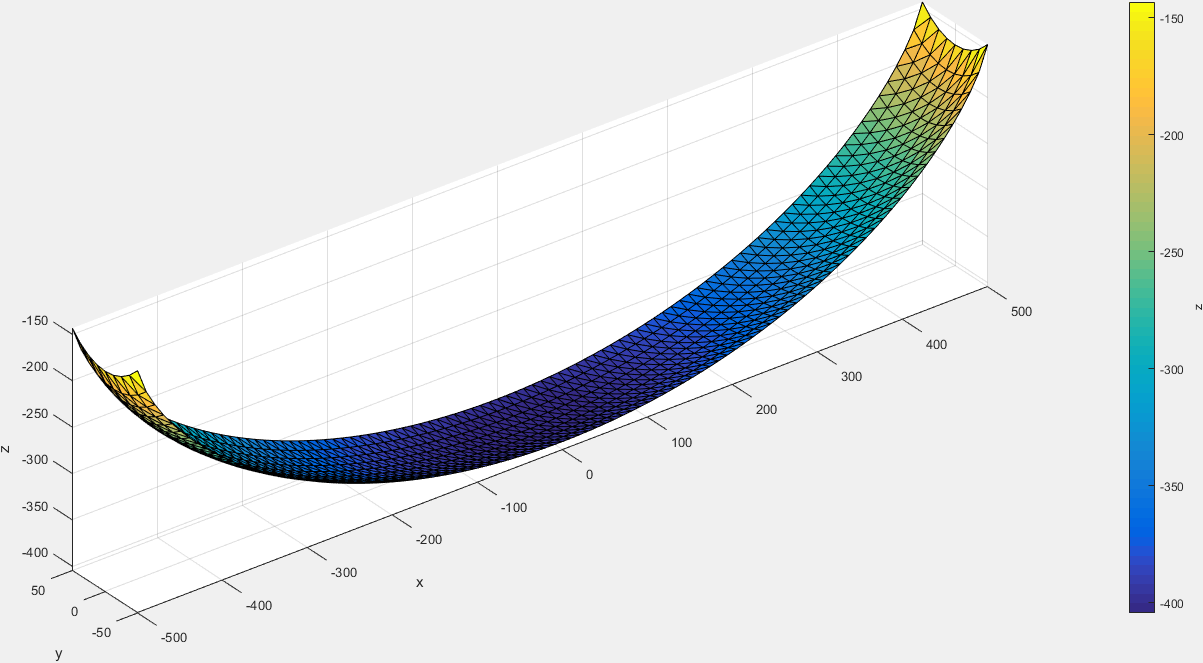
\includegraphics[width=\textwidth]{contsurf_rectangular_annualopt_surface}
\caption{the solar cell is located at z=0 and the light is travelling in positive z direction, continuopus surface, rectangular solar cell, optimised for annual improvement\label{contsurf_rectangular_annualopt_surface}}
\end{figure}

Similar to the previous chapter, it is useful to look at the average distance to the design point for normal incidence. This can be seen in figure \ref{contsurf_rectangular_annualopt_average_distance}. The colour indicates the distance to the design point. We can see that it performs bad for small and high y-values. This may be a result of the increase of the bending in y-direction. 

\begin{figure}[h]
\centering
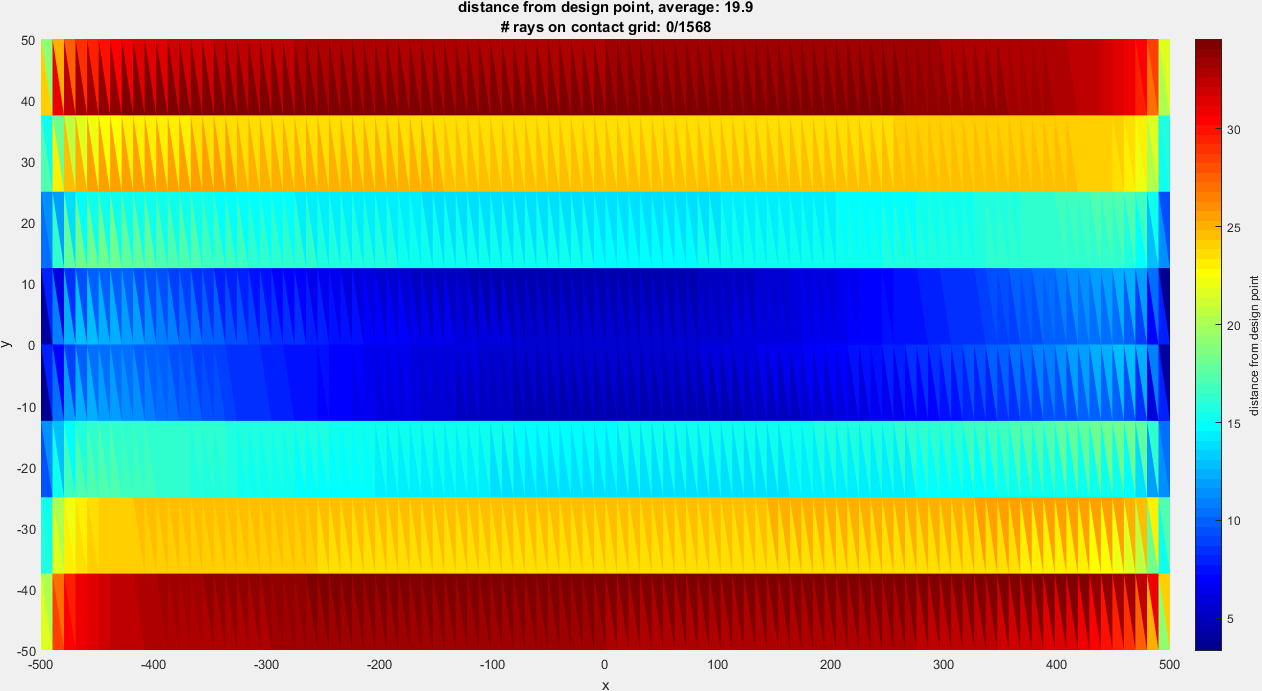
\includegraphics[width=\textwidth]{contsurf_rectangular_annualopt_average_distance.png}
\caption{shows the average distance to the designpoint,continuopus surface, rectangular solar cell, optimised for annual improvement \label{contsurf_rectangular_annualopt_average_distance}}
\end{figure}

However, we can read from table \ref{_table_rectangular_cell} that the annual improvement has increased to $11.01$ \%. This is 46.9 \% of the maximal annual improvement. In order to compute the annual improvement, we have to calculate the relative improvement for a few combinations of alpha/beta-values. It is important to take enough values in order to get precise values. By enough we mean a number of alphas/betas for which the annual improvement does stay approximately the same. To demonstrate this effect, we calculated the annual improvement for one parameter-set but two different precisions for the relative improvement. 
In figure \ref{contsurf_rectangular_annualopt_relative_improvement_dependant_of_alpha_and_beta} the relative improvement for different combinations of alpha and beta is shown. For different betas it works well. However, the relative improvement decreases rapidly around $beta=10 \deg$. The reason why we see sort of a periodic up and down for the relative improvement for a variation in alpha for beta=0 is because of the use of periodic boundary conditions. For alpha=12 and beta=0 a lot of rays are hitting the contact grid of the first cell. While increasing alpha, the rays are hitting the optic active area of the next solar cell and the relative improvement increases again. This periodic development does not happen for variation in beta. 
% KOMENTAR relative improvement stays the same looking at one plane

To sum up, the freeform surface design for a rectangular cell works up to maximal 46.9 \% of the maximal annual improvement. A cloak only in x-direction leads to an annual improvement of 43.7 \% of the maximal annual improvement. Comparing these two values, the gain of cloaking both directions is averaged over one year is 3.2 \%.  


\begin{figure}[h]
\centering
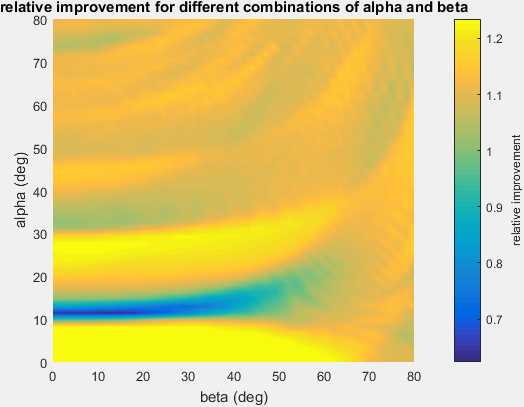
\includegraphics[width=\textwidth]{contsurf_rectangular_annualopt_relative_improvement_dependant_of_alpha_and_beta.png}
\caption{shows the relative improvement for different combinations of alpha and beta, notice that periodic boundary conditions are used to calculate the relative improvement, rectangular unit cell, parameters from optimised for annual improvement are used \label{contsurf_rectangular_annualopt_relative_improvement_dependant_of_alpha_and_beta}}
\end{figure}

\clearpage

\section{Simulation squared unit cell}

In the previous chapter we looked at a rectangular unit solar cell. It worked out that the cloaking in one direction (in x-direction) worked quite well but in y-direction it did not work well. One reason for this could be the asymmetric unit cell. Therefore, we decided to look at a squared unit cell. 

\subsection{Optimised for normal incidence}

Similar to the chapter \ref{SECTION_Simulation_rectangular_unit_cell} we optimised the parameter for normal incidence using the average distance and the number of rays hitting the contact grid as fitness. The surface optimised for normal incidence can be seen in figure \ref{contsurf_squared_normal_incident_surface}. We notice that the surface is approximately equally bend in x- and in y-direction. Keep in mind that the plots are not plotted with axis equal. 

\begin{figure}[h]
\centering
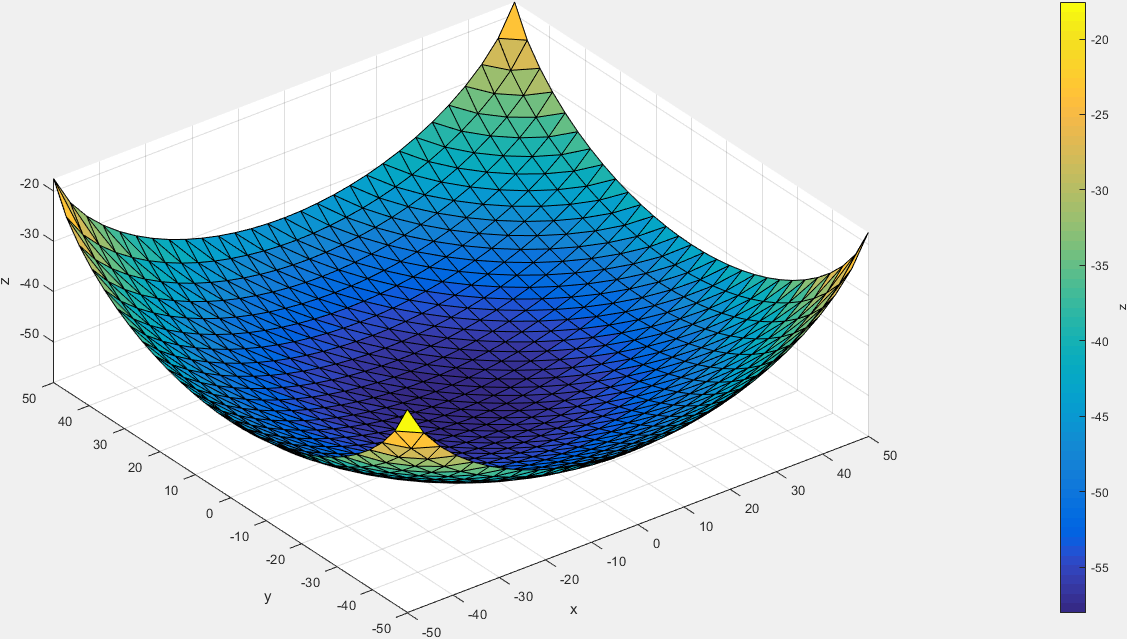
\includegraphics[width=\textwidth]{contsurf_squared_normal_incident_surface.png}
\caption{the solar cell is located at z=0 and the light is travelling in positive z direction, continuopus surface, squared unit cell, optimised for normal incidence \label{contsurf_squared_normal_incident_surface}}
\end{figure}

\begin{figure}[h]
\centering
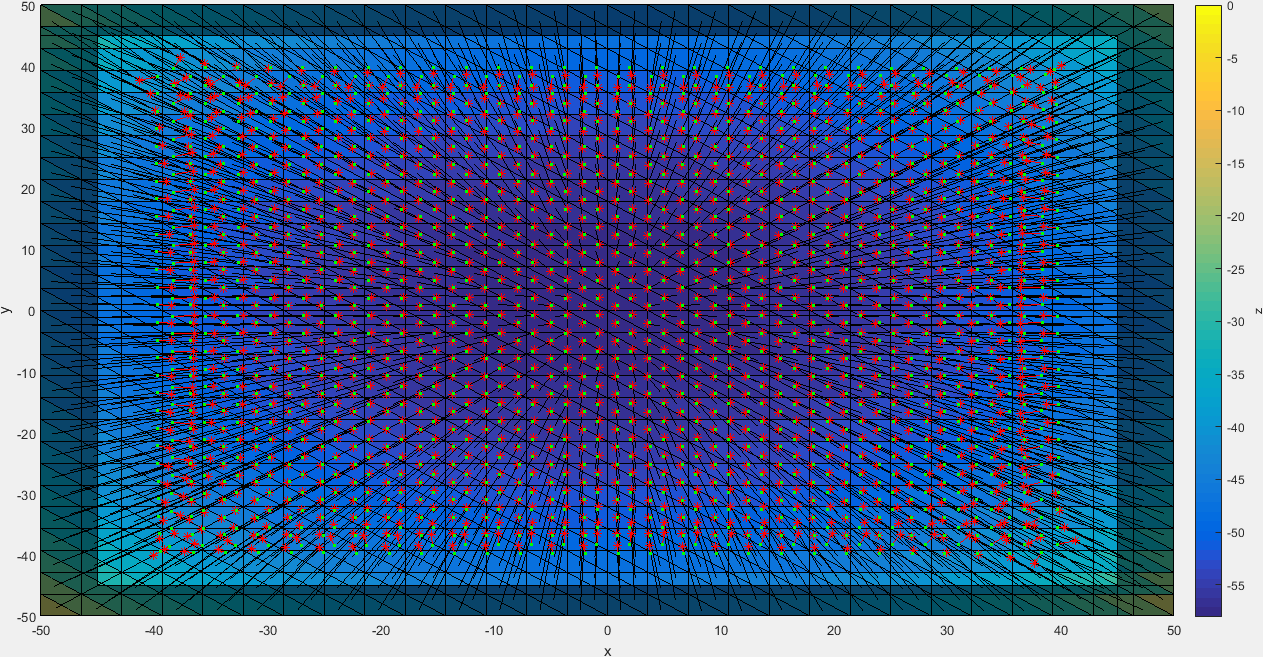
\includegraphics[width=\textwidth]{contsurf_squared_normal_incident_planeofsolarcell.png}
\caption{shows the average distance to the designpoint, continuopus surface, squared unit cell, optimised for normal incidence \label{contsurf_squared_normal_incident_planeofsolarcell}}
\end{figure}

Let us have a look at the projection to the plane of the solar cell. This can be seen in figure \ref{contsurf_squared_normal_incident_planeofsolarcell}. We can see that the design points and the points the rays hitting the solar cell fit nicely together. 


Figure \ref{contsurf_squared_normal_incident_average_distace} describes the quality of the design for normal incidence more quantitatively. No ray is hitting the contact grid and in addition to that, the average distance from the design point is 0.4. This is better than the average distance for the rectangular cell (1.3). We can also notice that within the precision of the calculations the average distance is symmetric. (due to triangulation it is not completely symmetric)

\begin{figure}[h]
\centering
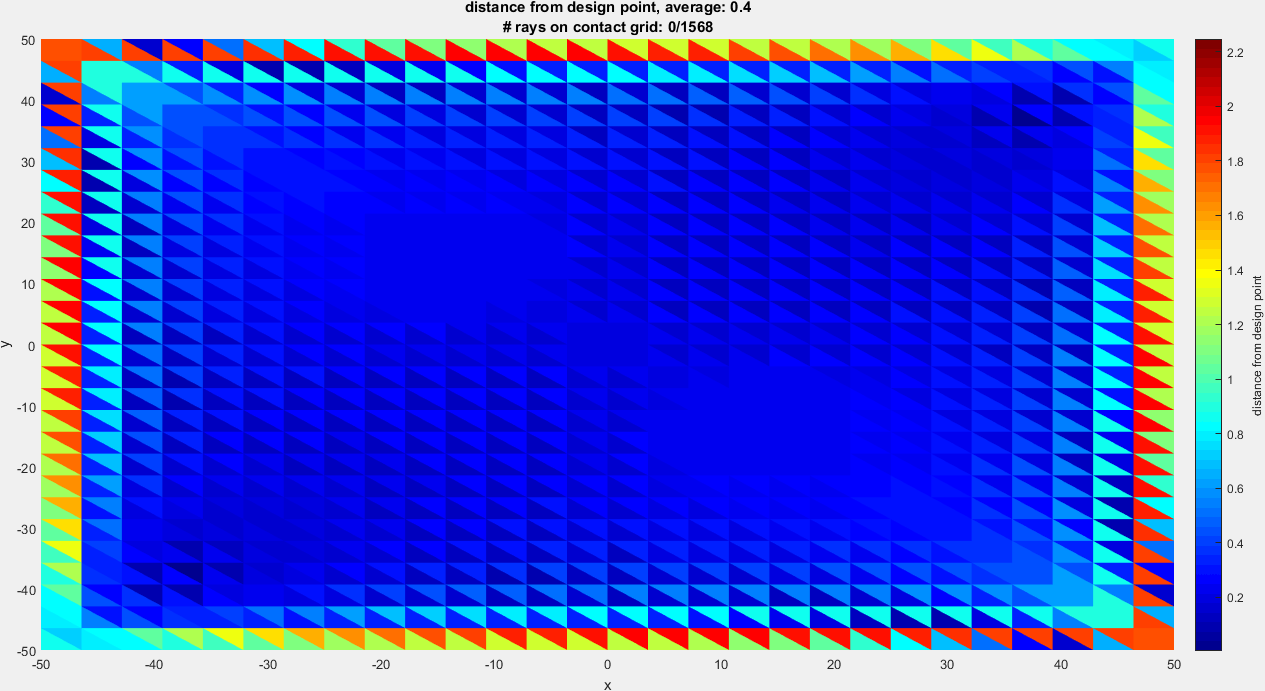
\includegraphics[width=\textwidth]{contsurf_squared_normal_incident_average_distace.png}
\caption{shows the average distance to the designpoint, continuopus surface, squared unit cell, optimised for normal incidence \label{contsurf_squared_normal_incident_average_distace}}
\end{figure}

The simulations for normal incident for the squared unit cell look promising. Calculating the annual improvement for this design only gives a annual improvement of 2.3 \% . This is about 9.5 \% of the maximal annual improvement. The parameters used for this calculation and the value for the annual improvement can be looked up in table \ref{_table_squared_cell}. 

\subsubsection{Optimised for annual improvement}

We optimised the squared design for annual improvement. (taking the annual improvement as fitness of the design) We reached a annual improvement of 11.5 \%. This is about 49.1 \% of the maximal annual improvement. This is a slightly better result as for rectangular unit cell. (as comparison 46.9 \% of maximal annual improvement for annual improvement optimisation for rectangular cell) 
The parameter-set for the squared unit cell can be found in table \ref{_table_squared_cell}. For a better understanding of the angular performance of the relative improvement, have a look at figure \ref{contsurf_squared_annualopt_relative_improvement_dependant_of_alpha_and_beta}. You can see the relative improvement for different values of alpha/beta-combinations. The plot looks more symmetric in alpha/beta than for the rectangular unit solar cell. 

\begin{table}
\centering
\caption{Parameters for simulation for squared unit cell ( 50 x 50 units) }
\label{_table_squared_cell}
\begin{tabular}{c|c|c|c|c|c|c}
a & b & y0x & y0y & $\xi$+1 & optimisation & [nalphas,nbetas] \\
\hline\hline
0.6 & 1.7 & 5.5 & 6.0 & 1.1153 & annualImpr. & [10,10] \\
1.9 & 1.9 & 9 & 9 & 1.0225 & normalinc. & [10,10] \\
1 & 0 & 5 & 0 & 1.1019 & only f(x) & [10,10] \\
0 & 1 & 0 & 5 & 1.1031 & only g(y) & [10,10]
\end{tabular}
\end{table}


\begin{figure}[h]
\centering
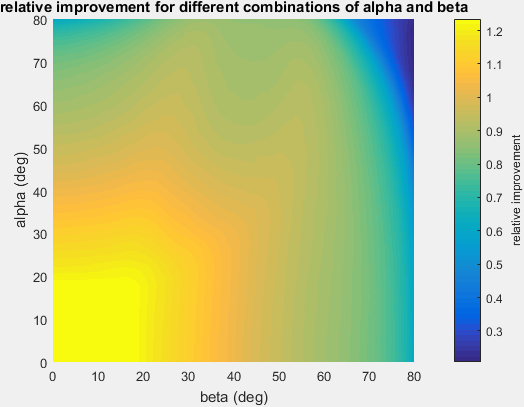
\includegraphics[width=\textwidth]{contsurf_squared_annualopt_relative_improvement_dependant_of_alpha_and_beta.png}
\caption{shows the relative improvement for different combinations of alpha and beta, notice that periodic boundary conditions are used to calculate the relative improvement, squared unit cell \label{contsurf_squared_annualopt_relative_improvement_dependant_of_alpha_and_beta}}
\end{figure}
